\documentclass[11pt]{report}

\special{papersize=8.5in,11in}

\topmargin -0.5in \oddsidemargin 0.00in \evensidemargin 0.00in
\textwidth 6.75in \textheight 9.0in \headheight 0.25in \headsep
0.25in \footskip 0.5in \hoffset 0in \marginparpush 0.0in
\marginparwidth 0.0in \marginparsep 0.2in

\setcounter{page}{1}

\newcommand{\D}{\displaystyle}\newcommand{\T}{\textstyle}
\newcommand{\e}{{\mathrm{exp}}}
\newcommand{\dd}{{\mathrm d}}
\newcommand{\comment}[1]{}
\newcommand{\mb}{\mathbf}
\reversemarginpar

\usepackage[final]{graphicx}
\usepackage{fancyhdr}
%\graphicspath{{Papers/}}
\usepackage{amsthm,amssymb,amsmath}
\usepackage{cite}
\usepackage{geometry}
\usepackage{amsmath}
\usepackage{booktabs}
\usepackage{color}
\usepackage{setspace}
\usepackage{subfigure}
\usepackage{url}
%\usepackage[top=2.5cm, bottom=2.5cm, right=3.5cm, left=3.5cm]{geometry}
\geometry{a4paper,scale=0.8}
\setcounter{secnumdepth}{3}

\title{Research Progress Report}

\author{Botao Zhu}

\begin{document}
	
	\maketitle
	\lhead{\sf Research Progress Report} \chead{} \rhead{\sf Botao Zhu}
	\lfoot{CTRG, University of Saskatchewan} \cfoot{} \rfoot{Page \thepage}
	\renewcommand{\footrulewidth}{1.0pt}
	\renewcommand{\headrulewidth}{2.0pt}
	\renewcommand{\arraystretch}{1.3}
	\pagestyle{fancy}
	
	\renewcommand{\thesection}{\arabic{section}}
	
	\section{Reading and Research Activities}
	
	\subsection{Summary}
	
	The existing networks structure and traffic control mechanisms are not adequate to cope with exponential increase in volume and complexity of the network traffic. \cite{8489985} proposed a reward based deep learning structure which jointly performs traffic load prediction and value based final action decision to control the network traffic in an intelligent manner to address the issues.
	
	\noindent For the supervised deep learning, some researchers proposed to train the network for packets forwarding based on labeled traffic data. However, the labeled traffic data are difficult to collect. In the non-supervised learning, the paths combinations are considered as the action space of the training process to choose the better action based on the action reward of each iteration. Such kind of path selection and action space design is reasonable only when the number of paths combination is finite. In order to solve the above issue, \cite{8489985} employs the set of next candidate forwarding destinations as the action space, and migrate the action decision process from the centralized controller to each distributed node. In addition, the reward are constructed as a vector to fit for the upcoming time sequences, which is able to more accurately measure the temporal connections between the selected action and get better computational cost performance than contemporary deep learning approaches.
	\begin{itemize}
		\item System model and action space format\\
		The topology of the considered network is a fully connected graph $G=\left(CR\cup AP,E\right)$, where $CR$ denotes the set of core routers in the network, $CR=\{cr_1,cr_2, \cdots, cr_{|CR|}\}$. AP denotes the set of access points, $AP=\left(ap_1,ap_2,\cdots,ap_{|AP|}\right)$, $N=|CR|+|AP|$, the total number of nodes, $E$ denotes the set of connection edges between all nodes. \\
		The action spaces is modeled and calculated as an algorithm complexity problem. Assuming the complexity of a single neural network is $\mathit{O}\left(1\right)$, 
	\end{itemize}
	
	\subsection{Deep Learning Based Routing Strategy}
	\subsubsection{Input and Output Design}
	
	\subsubsection{Deep Learning Structure Design}
	The authors choose the DBA as the deep learning structures as shown in Figure~\ref{1stfig}.
	\begin{figure}[h!]
		\centering
		%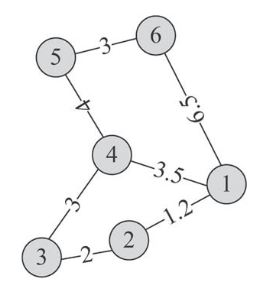
\includegraphics[width=0.5\linewidth]{figure1.png}
		\caption{Considered L-layer DBA}
		\label{1stfig}
	\end{figure}
	
	\subsubsection{The Procedures of the Proposed Deep Learning Based Routing Strategy}
	\paragraph{Initialization Phase}

	\paragraph{Training Phase}
     
	\begin{tabular}{lc}
		\toprule
		\textbf{Algorithm 1}. Supervised Train DBA\\
		\hline
		\textbf{Input:} $\left(x,y\right)=\{\left(x^t,y^t\right)|t=1,...,m\}, \eta_{CD}, \eta_{bp},L, n=\left(n_1,...,n_L\right)$\\
		\textbf{Output: $\theta$}\\
		1: \textbf{for} $i=1,...,L-2$ \textbf{do}\\
		2: \quad TrainRBM $\left(u^i,\eta_{CD},n_i,n_{i+1}\right)$\\
		3: \textbf{end for}\\
		4: Fine-tuneDBA$\left(\left(x,y\right),\theta,\eta_{bp}\right)$\\
		5: \textbf{return} $\theta$\\
		\hline
	\end{tabular}

	\paragraph{Running Phase} 

	
	\begin{table}[!h]
		\centering
		\caption{Routing table of $R_3$}
		\begin{tabular}{lc}
			\toprule
			Dest& Path\\
			\hline
			$R_1$& $R_3 \to R_2 \to R_1$\\
			$R_2$& $R_3 \to R_2$\\
			\dots& \dots\\
			$R_{16}$& $R_3 \to R_7 \to R_{11} \to R_{15} \to R_{16}$\\
			\hline
		\end{tabular}
	\end{table}

	
	\subsubsection{Network Performance Analysis}
	They compared the proposed deep learning method with OSPF by the network signaling overhead, throughput and average delay. 
	\begin{figure}[!htbp]
		%\centering
		\subfigure[Comparison of signaling overhead]{
			\begin{minipage}[t]{0.35\linewidth}
				\centering
			%	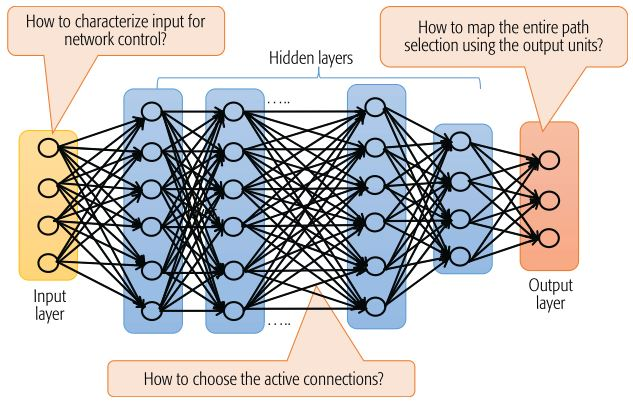
\includegraphics[width=2.4in]{figure5}
			\end{minipage}%
		}%
		\subfigure[Comparison of throughput]{
			\begin{minipage}[t]{0.35\linewidth}
				\centering
			%	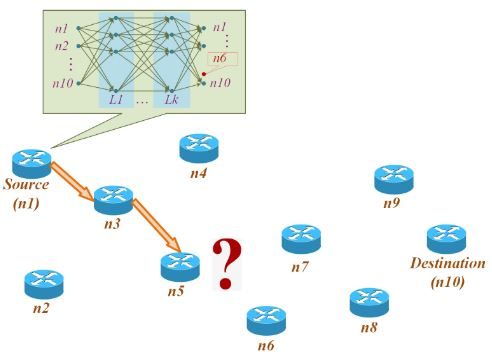
\includegraphics[width=2.4in]{figure6}
			\end{minipage}%
		}%
		\subfigure[Comparison of average delay]{
			\begin{minipage}[t]{0.35\linewidth}
				\centering
			%	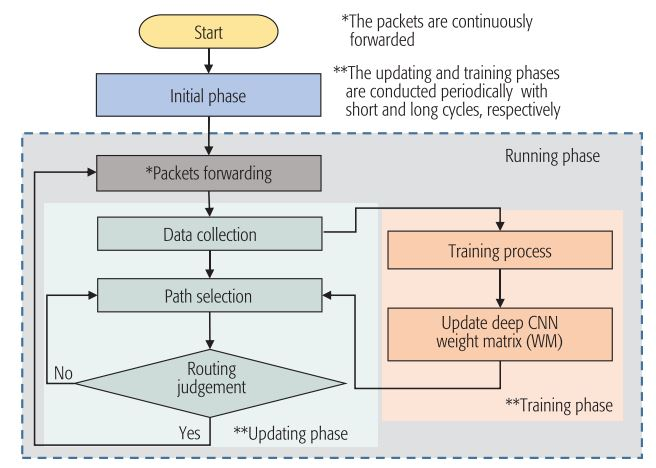
\includegraphics[width=2.4in]{figure7}
			\end{minipage}
		}%
	\centering
	\caption{Comparison of network performance under different network loads}
	\end{figure}
	
	\section{Objectives for the Next 2 Weeks}
	\subsection{Reading} 
	Reading papers foused on ML-based or DL-based routing.
	\subsection{Course} 
	Studying chapter 1 and chapter 2 of Neural Networks and Deep Learning, \textbf{Coursera}. \url{https://www.coursera.org/learn/neural-networks-deep-learning}
	\subsection{Code}
	Studying the classic routing protocol: LEACH and using Matlab to implement.
	
	\section{Advisor's Comments}
	
	\bibliographystyle{IEEEtran}
	\bibliography{janbib}
	
\end{document}